%--------------------------------------------------------------------%
%
% Berkas utama templat LaTeX.
%
% author Petra Barus, Peb Ruswono Aryan, Faris Rizki Ekananda, Fransiskus Febryan Suryawan
%
%--------------------------------------------------------------------%
%
% Berkas ini berisi struktur utama dokumen LaTeX yang akan dibuat.
%
%--------------------------------------------------------------------%

\documentclass[bahasa, 12pt, a4paper, onecolumn, oneside, final]{report}

%-------------------------------------------------------------------%
%
% Konfigurasi dokumen LaTeX untuk laporan tesis IF ITB
%
% @author Petra Novandi
%
%-------------------------------------------------------------------%
%
% Berkas asli berasal dari Steven Lolong
%
%-------------------------------------------------------------------%

% Ukuran kertas
\special{papersize=210mm,297mm}

% Setting margin
\usepackage[top=3cm,bottom=3cm,left=4cm,right=3cm]{geometry}

\usepackage{mathptmx}

% Judul bahasa Indonesia
\usepackage[bahasa]{babel}
\usepackage[bahasa]{translator}

% Format citation
\usepackage[utf8]{inputenc}

\usepackage[style=apa,backend=biber]{biblatex}
\usepackage{graphicx}
\usepackage{titling}
\usepackage{blindtext}
\usepackage{sectsty}
\usepackage{chngcntr}
\usepackage{etoolbox}
\usepackage[hidelinks]{hyperref}       % Package untuk link di daftar isi. Ubah jadi \usepackage[hidelinks]{hyperref} apabila ingin menghilangkan kotak merah disekitar link
\usepackage{titlesec}       % Package Format judul
\usepackage{titletoc}       % Package Format judul di toc
\usepackage{tocbibind}      % Package untuk masukkan toc, lot, lof ke Daftar Isi
\usepackage{scrwfile}       % Package untuk membuat Daftar Lampiran dari toc
\usepackage{parskip}
\usepackage{afterpage}
\usepackage{relsize}
\usepackage{amsmath}
\usepackage{amsfonts}
\usepackage{amssymb}
\usepackage{algpseudocode}
\usepackage{algorithm}
\usepackage{pgfgantt}
\usepackage[mode=buildnew]{standalone}


%--------------------------------------------------------------------%
%
% Hypenation untuk Bahasa Indonesia
%
% @author Petra Barus
%
%--------------------------------------------------------------------%
%
% Secara otomatis LaTeX dapat langsung memenggal kata dalam dokumen,
% tapi sering kali terdapat kesalahan dalam pemenggalan kata. Untuk
% memperbaiki kesalahan pemenggalan kata tertentu, cara pemenggalan
% kata tersebut dapat ditambahkan pada dokumen ini. Pemenggalan
% dilakukan dengan menambahkan karakter '-' pada suku kata yang
% perlu dipisahkan.
%
% Contoh pemenggalan kata 'analisa' dilakukan dengan 'a-na-li-sa'
%
%--------------------------------------------------------------------%

\usepackage{hyphenat}
\hyphenation {
	% A
	%
	a-na-li-sa
	a-pli-ka-si
	%
	% B
	%
	be-be-ra-pa
	ber-ge-rak
	%
	% C
	%
	ca-ri
	%
	% D
	%
	da-e-rah
	di-nya-ta-kan
	de-fi-ni-si
	%
	% E
	%
	e-ner-gi
	eks-klu-sif
	%
	% F
	%
	fa-si-li-tas
	%
	% G
	%
	ga-bung-an
	%
	% H
	%
	ha-lang-an
	%
	% I
	% 
	i-nduk
	% J
	%
	ka-me-ra
	kua-li-tas
	%
	% K
	%
	%
	% L
	%
	%
	% M
	%
	%
	% N
	%
	%
	% O
	%
	%
	% P
	%
	%
	% Q
	%
	%
	% R
	%
	%
	% S
	%
	%
	% T
	% 
	%
	% U
	%
	%
	% V
	%
	%
	% W
	%
	%
	% X
	%
	%
	% Y
	% 
	%
	% Z
	%
}

\usedictionary{translator-month-dictionary}

\graphicspath{{resources/}}   % letak direktori penyimpanan gambar

% Setting titik di daftar isi
\makeatletter
\renewcommand*{\@dotsep}{1.7}
\makeatother

% Setting daftar lampiran
\newcommand*{\lopname}{DAFTAR LAMPIRAN}
\TOCclone[\lopname]{toc}{atoc}
\addtocontents{atoc}{\protect\value{tocdepth}=-1}
\newcommand\listofappendices{
  \cleardoublepage
  \phantomsection
  \listofatoc
  \addcontentsline{toc}{chapter}{\lopname}
}

\newcommand*\savedtocdepth{}
\AtBeginDocument{%
  \edef\savedtocdepth{\the\value{tocdepth}}%
}

\let\originalappendix\appendix
\renewcommand\appendix{%
  \originalappendix
  \cleardoublepage
  \addtocontents{toc}{\protect\value{tocdepth}=-1}%
  \addtocontents{atoc}{\protect\value{tocdepth}=\savedtocdepth}%

  \titlecontents{chapter}
    [0pt]
    {\bfseries}
    {Lampiran \thecontentslabel.\quad}
    {}
    {\textmd{\dotfill}\contentspage}

  \titleformat{\chapter}[block]
    {\bfseries}
    {\chaptertitlename\ \thechapter.\quad}{0pt}
    {\bfseries}
}

% Setel title pada chapter-chapter di toc, lof, lot
\titlecontents{chapter}
  [0pt]
  {\bfseries}
  {\MakeUppercase{Bab} \thecontentslabel\quad\uppercase}
  {}
  {\textmd{\dotfill}\contentspage}
\titlecontents{figure}
  [0pt]
  {}
  {Gambar \thecontentslabel.\quad \enspace}
  {}
  {\dotfill\contentspage}
\titlecontents{table}
  [0pt]
  {}
  {Tabel \thecontentslabel.\quad \enspace}
  {}
  {\dotfill\contentspage}

% Masukin Daftar Pustaka ke toc
\let\originalprintbibliography\printbibliography
\renewcommand\printbibliography{%
  \phantomsection
  \cleardoublepage
  \originalprintbibliography
  \addcontentsline{toc}{chapter}{\bibname}
}

% Line satu setengah spasi
\renewcommand{\baselinestretch}{1.5}

% Setting judul
\chapterfont{\centering \Large}
\titleformat{\chapter}[display]
  {\Large\centering\bfseries}
  {\chaptertitlename\ \thechapter}{0pt}
    {\Large\bfseries\uppercase}

% Setting nomor pada subbsubsubbab
\setcounter{secnumdepth}{3}

\makeatletter

\makeatother

% Counter untuk figure dan table.
\counterwithin{figure}{section}
\counterwithin{table}{section}

% Define blank page
\newcommand*{\blankpage}{\afterpage{\null\newpage}}

% Define algorithm caption
\floatname{algorithm}{Algoritma}

% Definisi hyphen
\newcommand{\+}{\hyp}


\makeatletter

\makeatother

\addbibresource{references.bib}

\begin{document}

%Basic configuration
\title{PERANCANGAN DAN IMPLEMENTASI MODIFIKASI PENGOPTIMASI ADAM UNTUK \emph{DEEP LEARNING} TERDISTRIBUSI}
\date{}
\author{
    Fransiskus Febryan Suryawan \\
    NIM : 13519124
}

\pagenumbering{roman}
\setcounter{page}{1}

\clearpage
\pagestyle{empty}

\begin{center}
    \smallskip

    \Large \bfseries \MakeUppercase{\thetitle}
    \vfill

    \Large Laporan Tugas Akhir
    \vfill

    \large Disusun sebagai syarat kelulusan tingkat sarjana
    \vfill

    \large Oleh

    \Large \theauthor

    \vfill
    \begin{figure}[h]
        \centering
        
\includegraphics[width=0.15\textwidth]{cover-ganesha.jpg}
    \end{figure}
    \vfill

    \large
    \uppercase{
        Program Studi Teknik Informatika \\
        Sekolah Teknik Elektro \& Informatika \\
        Institut Teknologi Bandung
    }

    Desember 2022

\end{center}

\clearpage

\clearpage
\pagestyle{empty}

\begin{center}
    \smallskip
    
    \Large \bfseries \MakeUppercase{\thetitle}
    \vfill
    
    \Large Laporan Tugas Akhir I
    \vfill
    
    \large Oleh
    
    \Large \theauthor
    
    \large Program Studi Teknik Informatika \\
    
    \normalsize \normalfont
    Sekolah Teknik Elektro dan Informatika \\
    Institut Teknologi Bandung \\
    
    \vfill
    \normalsize \normalfont
    Bandung, 21 Oktober 2021 \\
    Mengetahui,
    
    \vspace{0.5cm}
    Pembimbing I,
    
    \vfill
    \underline{Nama dan Gelar Pembimbing I} \\
    NIP. 123456789
    
\end{center}
\clearpage
 % 1 PEMBIMBING PAKAI INI
% \clearpage
\pagestyle{empty}

\begin{center}
    \smallskip

    \Large \bfseries \MakeUppercase{\thetitle}
    \vfill

    \Large Laporan Tugas Akhir I
    \vfill

    \large Oleh

    \Large \theauthor

    \large Program Studi Teknik Informatika \\

    \normalsize \normalfont
    Sekolah Teknik Elektro dan Informatika \\
    Institut Teknologi Bandung

    \vfill
    \normalsize \normalfont
    Bandung, 21 Oktober 2021 \\
    Mengetahui,

    \vspace{0.5cm}
    \setlength{\tabcolsep}{12pt}
    \begin{tabular}{c@{\hskip 0.5in}c}
        Pembimbing I,                           & Pembimbing II,                           \\
                                                &                                          \\
                                                &                                          \\
                                                &                                          \\
                                                &                                          \\
        \underline{Nama dan Gelar Pembimbing I} & \underline{Nama dan Gelar Pembimbing II} \\
        NIP. 123456789                          & NIP. 123456789                           \\
    \end{tabular}

\end{center}
\clearpage
 % 2 PEMBIMBING PAKAI INI
% \chapter*{Lembar Pernyataan}

Dengan ini saya menyatakan bahwa:

\begin{enumerate}

    \item Pengerjaan dan penulisan Laporan Tugas Akhir ini dilakukan tanpa menggunakan bantuan yang tidak dibenarkan.
    \item Segala bentuk kutipan dan acuan terhadap tulisan orang lain yang digunakan di dalam penyusunan laporan tugas akhir ini telah dituliskan dengan baik dan benar.
    \item Laporan Tugas Akhir ini belum pernah diajukan pada program pendidikan di perguruan tinggi mana pun.

\end{enumerate}

Jika terbukti melanggar hal-hal di atas, saya bersedia dikenakan sanksi sesuai dengan Peraturan Akademik dan Kemahasiswaan Institut Teknologi Bandung bagian Penegakan Norma Akademik dan Kemahasiswaan khususnya Pasal 2.1 dan Pasal 2.2.
\vspace{15mm}

Bandung, 6 Juli 2015 \\
Petra Novandi \\
NIM 13505059


\pagestyle{plain}

% \clearpage
\chapter*{ABSTRAK}
\addcontentsline{toc}{chapter}{Abstrak}

%taruh abstrak bahasa indonesia di sini
Teknik \emph{Deep Learning} saat ini banyak digunakan untuk penyelesaian masalah dalam berbagai bidang. Salah satu contoh yang paling populer adalah ChatGPT, yang menggunakan model GPT milik OpenAI. Pembelajaran dalam \emph{deep learning} menggunakan proses stokastik atas \emph{dataset} yang ada untuk membuat aproksimasi fungsi tertentu. Model \emph{deep learning} memiliki beberapa \emph{layer}, yang masing-masing terdiri atas beberapa \emph{parameter}. Pengembangan model \emph{deep learning} umumnya dilakukan dengan menambah jumlah parameter dalam model.

Jumlah \emph{parameter} yang semakin banyak akan memengaruhi jumlah sumber daya yang diperlukan dalam pelatihan. Hal tersebut juga akan memengaruhi pembelajaran pada lingkungan terdistribusi. Pembelajaran dalam lingkungan terdistribusi memerlukan komunikasi, sehingga jumlah \emph{parameter} yang semakin banyak akan menyebabkan \emph{overhead} komunikasi meningkat.

Oleh karena itu, tugas akhir ini akan membahas serta menggabungkan teknik-teknik yang ada untuk mengurangi jumlah komunikasi dan ukuran data yang diperlukan untuk komunikasi dalam \emph{deep learning} terdistribusi. Teknik yang akan dikaji yakni teknik CADA dari \textcite{Chen2021CADA} serta Efficient-Adam dari \textcite{Chen2022Efficient}. Hasil penggabungan yang dilakuan memberikan pengurangan jumlah komunikasi yang lebih banyak dibandingkan CADA untuk model yang lebih besar, serta ukuran data yang cukup kecil dibandingkan teknik CADA.

Kata Kunci: \emph{deep learning} terdistribusi, modifikasi pengoptimasi Adam, kompresi bobot, pengurangan komunikasi
\clearpage

% \clearpage
\chapter*{Abstract}
\addcontentsline{toc}{chapter}{Abstract}

%put your abstract here
\blindtext

\clearpage
% \chapter*{Kata Pengantar}
\addcontentsline{toc}{chapter}{KATA PENGANTAR}

Puji serta syukur yang sebesar-besarnya penulis haturkan kepada Tuhan Yang Maha Esa, karena berkat karunia-Nya penulis mampu menyelesaikan tugas akhir dengan judul "Perancangan dan Implementasi Modifikasi Pengoptimasi Adam untuk \emph{Deep Learning} Terdistribusi" ini dengan baik. Tugas akhir ini juga tidak dapat selesai tanpa bantuan dari berbagai pihak, serta dukungan dari teman serta kerabat yang senantiasa mendorong penulis untuk terus melanjutkan pengerjaan tugas akhir ini. Oleh karena itu, penulis mengucapkan terima kasih sebesar-besarnya kepada:

\begin{enumerate}
  \item Bapak Achmad Imam Kistijantoro, S.T., M.Sc., Ph.D selaku dosen pembimbing tugas akhir yang telah memberikan banyak masukan berharga dalam penulisan buku tugas akhir ini,
  \item Seluruh dosen, staf pengajar, serta tata usaha Program Studi Teknik Informatika yang memberikan pengalaman, pengetahuan, serta bantuan dalam menempuh pendidikan sarjana hingga akhirnya mampu menulis tugas akhir ini,
  \item Keluarga penulis, yakni orang tua yang senantiasa memberikan dukungan terbesar kepada penulis selama menempuh pendidikan sarjana, serta saudara kandung penulis yang memberikan dukungan moral sehingga penulis tetap memiliki daya juang selama menulis tugas akhir ini, dan
  \item Teman-teman penulis yang terus memberikan dukungan moral serta menjadi pemacu dalam menulis tugas akhir agar penulis tidak merasa tertinggal, sehingga tugas akhir ini dapat selesai sesuai dengan rencana.
\end{enumerate}

Terakhir, penulis juga bersyukur atas adanya teman-teman satu hobi yang terus mendorong penulis untuk mencoba hal-hal baru dan keluar dari zona nyaman.


\titleformat*{\section}{\centering\bfseries\Large\MakeUpperCase}
\titlespacing*{\chapter}{0pt}{0pt}{3pc}

% Setting judul toc, lot, lof, bib
\renewcommand{\contentsname}{DAFTAR ISI}
\renewcommand{\listfigurename}{DAFTAR GAMBAR}
\renewcommand{\listtablename}{DAFTAR TABEL}
\renewcommand{\bibname}{DAFTAR PUSTAKA}

\tableofcontents
% \listofappendices
\listoffigures
% \listoftables

\newpage

\titleformat*{\section}{\bfseries\large}
\pagenumbering{arabic}

%----------------------------------------------------------------%
% Konfigurasi Bab
%----------------------------------------------------------------%
\setcounter{page}{1}
\renewcommand{\chaptername}{BAB}
\renewcommand{\thechapter}{\Roman{chapter}}
%----------------------------------------------------------------%

%----------------------------------------------------------------%
% Dafter Bab
% Untuk menambahkan daftar bab, buat berkas bab misalnya `chapter-6` di direktori `chapters`, dan masukkan ke sini.
%----------------------------------------------------------------%
\chapter{Pendahuluan}

\section{Latar Belakang}
\label{sec:latarbelakang}

Penggunaan teknik pembelajaran mesin pada saat ini banyak digunakan untuk menyelesaikan permasalahan dalam berbagai domain. Salah satu model pembelajaran mesin yang saat ini banyak digunakan adalah \emph{deep learning}. Proses dalam \emph{deep learning} meliputi pemrosesan atas \emph{dataset} yang dimiliki, kemudian membangun sebuah fungsi stokastik yang mampu memprediksi data yang tidak terdapat di \emph{dataset}.

Sebuah model \emph{deep learning} dibagi atas beberapa \emph{layer}, dan setiap \emph{layer} memiliki parameter yang dapat dioptimasi. Algoritma untuk mengoptimasi parameter\+parameter tersebut disebut sebagai \emph{backpropagation}, karena adanya rentetan pembaruan dari \emph{layer} terakhir hingga \emph{layer} pertama secara berurutan. Optimasi dari parameter-parameter tersebut akan menghasilkan fungsi stokastik yang mendekati fungsi sebenarnya dalam memprediksi \emph{dataset}.

Algoritma \emph{backpropagation} menggunakan gradien dari fungsi objektif untuk mengoptimasi parameter\+parameter. Algoritma pengoptimasi \emph{gradient descent} menggunakan hanya gradien untuk mengoptimasi parameter. Akibatnya, pengoptimasi tersebut mudah terjebak pada minimum lokal. Oleh sebab itu, perlu adanya faktor lain untuk membantu pengoptimasi agar tidak terjebak dalam minimum lokal.

Salah satu pengoptimasi yang umum digunakan dalam \emph{backpropagation} adalah Adam. Pengoptimasi Adam menggunakan gradien orde pertama dengan estimasi momen. Estimasi momen yang digunakan dapat membantu Adam untuk mencapai konvergensi lebih cepat, serta menghindari minimum lokal. Pengoptimasi tersebut memiliki kinerja yang baik pada permasalahan yang tidak konveks.

Dalam praktiknya, pembelajaran mesin dapat dilakukan dengan menjalankan perhitungan\+perhitungan yang sudah ditentukan. Namun, karena jumlah perhitungan dalam \emph{deep learning} meningkat dengan bertambahnya parameter, maka dibutuhkan suatu cara untuk mempercepat pembelajaran. Salah satu teknik awal yang dilakukan adalah dengan melakukan paralelisasi perhitungan menggunakan unit pemrosesan grafis atau GPU. Sebuah GPU mampu melakukan komputasi paralel dengan cepat dan efisien, sehingga cocok untuk melakukan perhitungan \emph{deep learning}.

Seiring berkembangnya model\+model \emph{deep learning}, semakin banyak parameter yang dimiliki model. Akibatnya, paralelisasi pada GPU saja tetap membutuhkan waktu yang signifikan untuk melakukan optimasi parameter. Oleh karena itu, paralelisasi kemudian dilakukan pada beberapa mesin dengan GPU terpisah. Dengan melakukan pembelajaran pada beberapa mesin, parameter dapat dioptimasi dengan lebih cepat.

Selain masalah jumlah parameter, ukuran \emph{dataset} yang digunakan juga menjadi faktor dalam pembelajaran. Saat ini, tersedia beragam \emph{dataset} yang memiliki ukuran besar. Sebuah GPU memiliki jumlah memori yang terbatas, sehingga tidak mungkin memuat keseluruhan \emph{dataset}. Oleh karena itu, akan lebih baik apabila jumlah \emph{dataset} dapat dikurangi dengan membaginya ke beberapa mesin.

Paralelisasi perhitungan dalam \emph{deep learning} dapat mempercepat proses pembelajaran yang dilakukan. Oleh karena itu, banyak penelitian yang meninjau optimasi dalam menggunakan sistem terdistribusi. Aspek penting yang ditinjau adalah mengurangi jumlah komunikasi sehingga mesin tidak banyak menunggu. Salah satu bagian yang mempengaruhi jumlah komunikasi antar \emph{worker} adalah pengoptimasi yang digunakan serta aturan pembaruan bobot.

Penelitian dari \textcite{Chen2021CADA} memberikan alternatif pembaruan bobot dalam lingkungan terdistribusi dengan menggunakan kriteria tertentu untuk menentukan \emph{worker} yang harus mengirimkan parameter dan \emph{worker} yang tidak perlu mengirimkan parameter. Aturan pembaruan ini dapat mengurangi jumlah komunikasi yang diperlukan, namun tetap menjamin konvergensi model. Akibatnya, pembelajaran dapat dilakukan dengan lebih efisien.

Penelitian lain dari \textcite{Chen2022Efficient} memberikan alternatif untuk mengurangi beban komunikasi dengan mengurangi data yang dikirimkan. Ukuran data dikurangi dengan cara melakukan kuantisasi. Untuk mengatasi masalah bias, \textcite{Chen2022Efficient} menggunakan \emph{error\+feedback}. Akibatnya, beban komunikasi dapat dikurangi.

\section{Rumusan Masalah}
Algoritma pengoptimasi Adam dalam lingkungan terdistribusi memiliki banyak modifikasi. Beberapa yang telah disebutkan yakni algoritma dari \textcite{Chen2021CADA} serta \textcite{Chen2022Efficient}. Algoritma dari \textcite{Chen2021CADA} mengoptimasi komunikasi dengan mengurangi jumlah komunikasi. Algoritma dari \textcite{Chen2022Efficient} mengoptimasi komunikasi dengan mengurangi ukuran data yang dikirimkan saat komunikasi.

Belum ada modifikasi pengoptimasi Adam yang secara bersamaan mengurangi jumlah komunikasi dan ukuran data yang dikirimkan. Maka, rumusan masalah dari tugas akhir ini ialah:

\begin{enumerate}
    \item Bagaimana cara memodifikasi pengoptimasi Adam pada lingkungan terdistribusi sehingga ukuran data dan jumlah komunikasi dapat dikurangi?
    \item Bagaimana perbandingan jumlah komunikasi dari modifikasi tersebut terhadap algoritma dari \textcite{Chen2021CADA}?
    \item Bagaimana perbandingan ukuran data dari modifikasi tersebut terhadap algoritma dari \textcite{Chen2022Efficient}?
\end{enumerate}

\section{Tujuan}

Berdasarkan rumusan masalah yang telah ditulis pada subbab sebelumnya, tujuan dari tugas akhir ini ialah:
\begin{enumerate}
    \item Melakukan modifikasi terhadap pengoptimasi Adam pada lingkungan terdistribusi untuk mengurangi ukuran data dan jumlah komunikasi.
    \item Melakukan analisis komparatif dengan algoritma dari \textcite{Chen2021CADA}.
    \item Melakukan analisis komparatif dengan algoritma dari \textcite{Chen2022Efficient}.
\end{enumerate}

% \section{Batasan Masalah}

% Adapun batasan masalah yang ditetapkan untuk tugas akhir ini ialah:
% \begin{enumerate}
%     \item Analisis akan dilakukan terhadap simulasi, sehingga tidak dilakukan pada lingkungan terdistribusi yang nyata.
% \end{enumerate}

\section{Metodologi}

Metodologi yang digunakan dalam tugas akhir ini ialah:
\begin{enumerate}
    \item Mempelajari metode yang digunakan pada penelitian \textcite{Chen2021CADA} dan \textcite{Chen2022Efficient}.
    \item Pengembangan modifikasi Adam menggunakan teknik yang digunakan pada penelitian \textcite{Chen2021CADA} dan \textcite{Chen2022Efficient}.
    \item Melakukan implementasi terhadap modifikasi yang dibuat.
    \item Melakukan pengujian terhadap implementasi.
\end{enumerate}

\section{Jadwal Pelaksanaan Tugas Akhir}

Rencana jadwal pelaksanaan tugas akhir dapat dilihat pada gambar~\ref{jadwalTA1} dan gambar~\ref{jadwalTA2}.


\begin{figure}[H]
    \includestandalone[width=\textwidth]{figures/gantt-1}
    \caption{
        \label{jadwalTA1}
        Jadwal pelaksanaan Tugas Akhir 1
    }
\end{figure}

\begin{figure}[H]
    \includestandalone[width=\textwidth]{figures/gantt-2}
    \caption{
        \label{jadwalTA2}
        Jadwal pelaksanaan Tugas Akhir 1
    }
\end{figure}

\chapter{Studi Literatur}
Pada bab ini, akan dikaji literatur yang terkait \emph{Deep Learning} Terdistribusi. Pokok bahasan utama dalam bab ini adalah teori yang mendasari \emph{Deep Learning}, yang merujuk kepada \textcite{JiangDistributed}, \textcite{Choi2019}, \textcite{Fan2019}, serta \textcite{LeCun2015}. Kemudian, akan dibahas pula implementasi \emph{Deep Learrning} Terdistribusi yang ada saat ini.

\section{Machine Learning}
Berdasarkan literatur \textcite{Fan2019} serta \textcite{bishop2006pattern}, teknik \emph{Supervised Machine Learning} modern mencari suatu fungsi dengan mempelajari himpunan \emph{training data} $\{(x_i, y_i)\}_{1 \le i \le n}$, dimana $x_i \in \mathbb{R}^d$ disebut sebagai fitur,  $y_i \in \mathbb{R}$ disebut sebagai label, dan $n$ merupakan jumlah \emph{training data} yang akan dipelajari. Dari \emph{training data} tersebut, akan dicari fungsi $f: \mathbb{R}^d \mapsto \mathbb{R}$ dari kelas fungsi $\mathcal{F}$ yang dapat memprediksi \emph{output} $y_i$ berdasarkan \emph{input} $x_i$ dengan baik.

Terdapat beragam kelas fungsi \(\mathcal{F}\) yang dapat dipilih untuk mempelajari himpunan \emph{training data}. Contoh teknik terkait adalah regresi linear yang menggunakan kelas fungsi linear untuk mempelajari \emph{training data}. Selain itu, terdapat pula teknik \emph{deep learning} yang menggunakan kelas komposisi fungsi \parencite{LeCun2015}
\begin{equation}
  \{
  f(x;\theta) = W_L\sigma_L(W_{L-1} \cdots \sigma_2(W_2\sigma_1(W_1 x)))\ \vert \ \theta = \{W_1,\dots,W_L\}
  \}
\end{equation}
dimana $L$ menyatakan jumlah \emph{layer} yang umumnya disebut sebagai kedalaman sebuah model, $W_i$ merupakan bobot untuk keluaran fungsi ke-$i$, dan fungsi $\sigma_i$ merupakan fungsi aktivasi ke-$i$.

\section{Deep Learning}
Istilah \emph{deep learning} atau \emph{deep neural network} digunakan secara umum untuk menggambarkan sebuah model \emph{neural network} yang memiliki satu atau lebih \emph{hidden layer} \parencite{Fan2019,LeCun2015}. Struktur model \emph{neural network} dapat mengandung sebuah \emph{input layer}, beberapa \emph{hidden layer}, dan sebuah \emph{output layer}.

Menurut \textcite{Bengio2021}, struktur model yang memiliki beberapa lapisan fungsi memungkinkan model untuk mempelajari data yang tidak linear. Selain itu, model yang lebih dalam memungkinkan adanya transformasi fitur menjadi lebih abstrak dalam komposisi fungsi, yang kemudian dapat digunakan oleh \emph{layer} Selanjutnya.

\subsection{Model Deep Neural Network}
Model \emph{deep neural network} merupakan komposisi dari beberapa fungsi aktivasi nonlinear $\sigma$. Untuk layer ke-$l$, \emph{output} yang dihasilkan adalah

\begin{equation}
  h^{(l)} = g^{(l)}(h^{(l-1)}) = \sigma(W^{(l)}h^{(l-1)} + b^{(l)}),
\end{equation}

dengan $l \in \{1,2,\dots,L\}$, $h^{(0)} = x$, $W^{(l)}$ adalah matriks bobot, dan $b^{(l)}$ adalah matriks bias untuk \emph{layer} ke-$l$.

Beberapa fungsi yang umumnya digunakan sebagai fungsi aktivasi $\sigma$ adalah \emph{Rectified Linear Unit} (ReLU), \emph{sigmoid}, dan tanh. Selain itu, untuk \emph{output} multilabel atau lebih dari dua label, digunakan fungsi softmax pada \emph{output layer} untuk menghitung probabilitas dari fungsi linear. Definisi fungsi softmax adalah sebagai berikut:
\begin{equation}
  softmax(z_k) \triangleq \frac{\exp(z_k)}{\Sigma_k \exp(z_k)},
  k \in \{1,\dots,K\}
\end{equation}
dengan $K$ adalah kategori klasifikasi yang mungkin.

Hasil dari \emph{Deep Learning} adalah sebuah fungsi penebak $\hat{f}$. Kinerja sebuah fungsi penebak $\hat{f}$ dapat dievaluasi menggunakan galat prediksi $\mathbb{P}(y \neq \hat{f}(x))$.

\subsection{Algoritma Backpropagation}
Pembelajaran yang dilakukan di dalam \emph{deep learning} adalah meminimasi fungsi objektif yang didefinisikan. Definisi fungsi objektif dapat dibuat dengan membandingkan hasil dari \emph{output layer} $h^{(L)}$ dengan label sebenarnya $y$. Fungsi objektif yang umum digunakan untuk masalah klasifikasi adalah \emph{multinomial logistic loss} yang didefinisikan sebagai
\begin{equation}
  \mathcal{L}(f(x;\theta),y) = -\sum_{k=1}^K 1\{y=k\} \log p_k,
\end{equation}
dimana $x$ adalah input, $y$ adalah label seharusnya, $K$ adalah jumlah kelas yang digunakan, $p_k$ adalah keluaran kemungkinan input $x$ berada dalam kelas $k$ menurut fungsi $f$.

Gradient descent merupakan cara untuk meminimasi fungsi objektif $J(\theta)$ yang diparameterisasi oleh parameter model $\theta \in \mathbb{R}^d$. Algoritma ini memperbarui parameter ke arah berlawanan dari arah gradien fungsi objektif $\nabla_\theta J(\theta)$ terhadap parameternya.

Karena \emph{deep neural network} memiliki beberapa \emph{hidden layer}, maka diperlukan aturan rantai untuk menghitung gradien. Perhitungan gradien dilakukan dari \emph{output layer} dan dipropagasi balik ke \emph{layer} sebelumnya. Nilai gradien untuk \emph{layer} ke-$l-1$ dapat dihitung sebagai berikut:
\begin{equation}
  \frac{\partial J}{\partial h^{(l-1)}}
  = \frac{\partial h^{(l)}}{\partial h^{(l-1)}}
  \frac{\partial J}{\partial h^{(l)}}
  = \frac{\partial \sigma(W^{(l)} h^{(l-1)} + b^{(l)})}{\partial h^{(l-1)}}
  \frac{\partial J}{\partial h^{(l)}}
\end{equation}

Gradien tersebut kemudian dapat digunakan untuk memperbarui matriks bobot:
\begin{equation}
  W^{(l)} \leftarrow W^{(l)}
  - \eta \frac{\partial J}{\partial W^{(l)}}
  \text{, dimana }
  \frac{\partial f}{\partial W^{(l)ij}}
  = \frac{\partial f}{\partial h_i^{(l)}}\sigma'h_j^{(l-1)}
\end{equation}
Nilai $\eta > 0$ disebut sebagai \emph{learning rate}, yang mengatur seberapa jauh setiap parameter diubah dalam satu langkah pembaruan.

Nilai $\eta$ beserta jumlah parameter dalam $\theta$ dapat dikategorikan sebagai \emph{hyperparameter} yang dapat diatur untuk menentukan model \emph{deep neural network} yang dibangun. Dalam beberapa literatur, nilai \emph{learning rate} umumnya dituliskan sebagai $\alpha$.

\subsection{Optimasi Untuk Gradient Descent}
Terdapat beberapa varian dari gradient descent untuk menghitung gradien, yang dikarakterisasi oleh jumlah data yang digunakan. Varian pertama memperbarui parameter untuk setiap keseluruhan \emph{training data}, disebut sebagai \emph{batch gradient descent}. Kemudian, varian kedua menggunakan hanya satu data untuk memperbarui parameter, yang disebut sebagai \emph{stochastic gradient descent}(SGD). Varian ketiga menggunakan sebagian \emph{training data} untuk memperbarui parameter, sehingga disebut \emph{mini-batch gradient descent}. Ketiga varian tersebut memberikan pertukaran antara kecepatan pembaruan dan akurasi pembaruan.

Algoritma optimasi (selanjutnya disebut pengoptimasi) untuk gradient descent dirancang untuk mencoba menyelesaikan tantangan-tantangan yang ada pada gradient descent. Selain itu, pengoptimasi yang dirancang juga dapat mempercepat konvergensi model \emph{deep neural network} pada saat pembelajaran. Oleh karena itu, penting untuk memilih pengoptimasi yang tepat untuk pembelajaran sebuah model \emph{deep neural network}.

Terdapat beberapa pengoptimasi yang dapat digunakan dalam pelatihan model \emph{deep neural network}. Beberapa pengoptimasi yang disebutkan oleh \textcite{Ruder2016} diantaranya adalah Momentum dari \textcite{qian1999momentum}, RMSProp dari \textcite{hinton2012neural}, Adam dari \textcite{ADAMKingma}, serta pengoptimasi lainnya. Perbandingan empiris antar pengoptimasi telah dilakukan oleh banyak penulis sebelumnya. Menurut \textcite{Choi2019}, pengoptimasi yang lebih umum tidak akan memiliki kinerja yang lebih buruk dibandingkan pengoptimasi yang lebih khusus. Hasil perbandingan yang dilakukan \textcite{benchmark2021schmidt} menyatakan Adam merupakan salah satu pilihan yang cukup baik untuk banyak permasalahan, dengan alternatif lain yakni \emph{Nesterov Accelerated Gradient}(NAG) dan RMSProp.

\subsection{Pengoptimasi RMSProp}
Pengoptimasi RMSProp dituliskan oleh \textcite{hinton2012neural} untuk mendemonstrasikan momentum per parameter dalam pengoptimasi SGD. Dalam tulisan tersebut, ditawarkan sebuah cara untuk memberikan \emph{learning rate} yang berbeda untuk setiap parameter. Salah satu cara yang ditulis untuk menentukan \emph{learning rate} masing-masing parameter adalah menggunakan \emph{local gain} $g(t)$ yang diinisialisasi menjadi 1 untuk setiap parameter. Kemudian, \emph{local gain} akan diperbarui dengan aturan berikut.
\begin{equation*}
  g(t) =
  \begin{cases}
    g(t-1) + 0.5      & \text{, jika } \left(
    \frac{\partial J}{\partial w}(t) \frac{\partial J}{\partial w}(t-1) > 0
    \right)                                   \\
    g(t-1) \cdot 0.95 & \text{, lainnya}
  \end{cases}
\end{equation*}
Namun, aturan tersebut kurang baik untuk \emph{mini-batch gradient descent}, sehingga perlu adanya sebuah bilangan pembagi yang mendekati gradien \emph{mini-batch} yang berdekatan. Oleh karena itu, digunakan sebuah rerata bergerak dari kuadrat gradien setiap parameter.
$$
  MeanSquare(w, t) = 0.9 MeanSquare(w, t-1) + 0.1\left(\frac{\partial J}{\partial w}(t)\right)^2
$$

\subsection{Pengoptimasi Adam}
\begin{algorithm}
  \setstretch{1}
  \caption{Algoritma Pengoptimasi Adam}\label{Adam}
  \begin{algorithmic}[1]
    \Function{Adam}{$\alpha$, $\beta_1$, $\beta_2$, $\theta_0$}
    \State $m_0 \gets 0$ \Comment{Inisialisasi estimasi momen pertama}
    \State $v_0 \gets 0$ \Comment{Inisialisasi estimasi momen kedua}
    \State $t \gets 0$ \Comment{Inisialisasi \emph{timestep}}
    \While{$\theta_t$ not converged}
    \State $t \gets t+1$
    \State $g_t \gets \nabla_\theta f_t (\theta_{t-1})$
    \State $m_t \gets \beta_1 \cdot m_{t-1} + (1 - \beta_1) \cdot g_t$ \Comment{Perbarui estimasi momen pertama terbias}
    \State $v_t \gets \beta_2 \cdot v_{t-1} + (1-\beta_2) \cdot g_t^2$ \Comment{Perbarui estimasi momen kedua terbias}
    \State $\hat{m_t} \gets m_t/(1-\beta_1^t)$ \Comment{Hitung estimasi momen pertama dengan perbaikan bias}
    \State $\hat{v_t} \gets v_t/(1-\beta_2^t)$ \Comment{Hitung estimasi momen kedua dengan perbaikan bias}
    \State $\theta_t \gets \theta_{t-1} - \alpha \cdot \hat{m_t}/\sqrt{\hat{v_t}}+\epsilon$
    \EndWhile
    \State \textbf{return} $\theta_t$ \Comment{Parameter hasil optimasi}
    \EndFunction
  \end{algorithmic}
\end{algorithm}

Tulisan dari \textcite{ADAMKingma} menjelaskan sebuah algoritma untuk mengoptimasi SGD menggunakan hanya gradien orde pertama. Pengoptimasi tersebut menghitung \emph{learning rate} adaptif untuk setiap parameter menggunakan estimasi momen orde pertama dan kedua dari gradiennya. Penggunaan momen dapat membantu pengoptimasi agar tidak terjebak pada minimum lokal.

Algoritma yang dijelaskan dalam literatur tersebut menggunakan estimasi momen pertama dan kedua, yakni $m_t$ dan $v_t$. Parameter $\beta_1$ dan $\beta_2$ sebagai laju peluruhan untuk estimasi momen. Keduanya menjadi \emph{hyperparatemer} yang dapat diatur, bersama dengan \emph{hyperparameter} lain dari SGD. Literatur tersebut memberikan nilai-nilai dasar yang cukup baik untuk \emph{hyperparameter} yang ada, yakni $\beta_1 = 0.9$, $\beta_2 = 0.999$, $\alpha = 0.001$. Selain itu, nilai $\epsilon$ yang digunakan adalah $\epsilon = 10^{-8}$

Hasil analisis dari \textcite{ADAMKingma} menunjukkan \emph{stepsize} yang digunakan akan mendekati nol apabila fungsi objektif mendekati optimum. Selain itu, terdapat perbaikan bias untuk momen pertama dan kedua agar tidak terbias menuju nol.

\section{Distributed Deep Learning}
Pembelajaran dalam \emph{deep learning} membutuhkan komputasi yang banyak, terutama ketika jumlah parameter yang harus dioptimasi mencapai lebih dari jutaan. Oleh karena itu, pembelajaran \emph{deep neural network} kemudian dilakukan secara terdistribusi untuk mempercepat proses. Namun, terdapat beberapa masalah mendasar untuk membuat pembelajaran \emph{deep neural network} dapat dilakukan secara terdistribusi. Pertama, bagaimana komputasi akan diparalelisasi. Kedua, bagaimana mengagregasi parameter dari hasil pembelajaran. Ketiga, bagaimana mensinkronisasi \emph{worker} yang menjalankan \emph{deep learning}. Keempat, bagaimana mengoptimasi komunikasi selama pembelajaran.

\subsection{Optimasi komunikasi}
Untuk membagi parameter ke \emph{worker} yang terdistribusi, beberapa \emph{parameter server} dapat digunakan. Sebuah \emph{parameter server} bertugas membagikan parameter dan mengagregasi kembali parameter baru yang dihitung oleh \emph{worker}. Penggunaan beberapa \emph{parameter server} dapat meringankan beban setiap \emph{parameter server}. Dalam skema ini, setiap parameter baru harus dikirimkan ke \emph{parameter server} sehingga semua model dapat mengetahui parameter terbaru. Hal tersebut penting untuk konvergensi \emph{deep neural network}.

Skema kompresi pada parameter dapat digunakan untuk mengoptimasi komunikasi lebih jauh. Beberapa kompresi yang umum dilakukan adalah kompresi \emph{lossless} untuk bilangan bulat (\emph{integer}) dan matriks jarang (\emph{sparse matrices}). Kemudian, terdapat pula kompresi \emph{lossy} untuk bilangan real yang dinyatakan dalam bentuk \emph{floating point}. Algoritma kompresi seperti yang dikembangkan \textcite{Jin2021Comet} dan \textcite{Horvoth2022Natural} dapat melakukan kompresi \emph{lossy} untuk mengoptimasi komunikasi dan penggunaan memori saat pembelajaran.

\subsection{Pengoptimasi pada Deep Learning Terdistribusi}
Pengoptimasi yang disebutkan sebelumnya dikembangkan untuk digunakan pada lingkungan yang terpusat. Oleh karenanya, terdapat penelitian lebih lanjut untuk meninjau pengoptimasi yang ada ketika digunakan dalam lingkungan terdistribusi. Salah satu pengoptimasi yang sebelumnya telah disebutkan sebagai alternatif yang cukup baik adalah pengoptimasi Adam. Terdapat banyak pengembangan untuk mengoptimasi Adam di lingkungan terdistribusi, umumnya dengan melakukan kompresi seperti dilakukan oleh \textcite{Chen2021CADA}. Selain itu, terdapat pula algoritma yang mengurangi jumlah komunikasi yang diperlukan, seperti ditulis oleh \textcite{Li2022Federated} dan \textcite{Chen2021CADA}.

\section{Penelitian Terkait}

\subsection{Pengurangan Komunikasi}
Komunikasi antar \emph{worker} menjadi sebuah pembatas kecepatan pembelajaran. Pengurangan jumlah sinkronisasi dapat mempercepat proses pembelajaran, namun perlu ditinjau terlebih dahulu efeknya terhadap konvergensi model. Penelitian \textcite{Chen2018LAG} memberikan alternatif solusi, yakni \emph{lazily aggregated gradient} untuk mengurangi komunikasi. Teknik yang digunakan adalah dengan memilih \emph{worker} yang perlu mengirimkan gradien melalui kriteria tertentu. Kriteria yang diberikan dievaluasi pada setiap \emph{worker}, namun apabila \emph{broadcast} dianggap berat maka kriteria dapat dievaluasi pada \emph{parameter server}.

Pengurangan yang diberikan oleh \textcite{Chen2018LAG} dapat mempercepat proses pembelajaran. Akan tetapi, \textcite{Chen2021CADA} meninjau bahwa keefektifan dari algoritma tersebut akan berkurang seiring berjalannya pembelajaran. penelitian \textcite{Chen2021CADA} memberikan alternatif lain untuk mengurangi jumlah komunikasi yang diperlukan. Algoritma tersebut, yang diberi tajuk \emph{CADA}, memiliki kriteria yang berbeda dari \emph{lazily aggregated gradient}, dan telah ditunjukkan akan konvergen pada kondisi yang sesuai.

Dalam CADA, pembaruan parameter dilakukan dengan mengambil gradien baru hanya dari sebagian \emph{worker}, sedangkan \emph{worker} lainnya akan menggunakan gradien sebelumnya. Terdapat dua varian CADA dengan kondisi yang berbeda. Kedua varian kondisi dapat dilihat pada \autoref{CADA1} dan \autoref{CADA2}. Dalam kedua kondisi, \emph{worker} akan mengirimkan gradien apabila \autoref{CADA1} atau \autoref{CADA2} tidak terpenuhi. Kondisi tersebut dievaluasi pada setiap \emph{worker} untuk setiap \emph{iterasi}.

\begin{equation}
  \label{CADA1}
  \|\tilde{\delta}_t^{(i)} - \tilde{\delta}^{(i)}_{\tau_t^{(i)}}\|^2 \leq \frac{c}{d_{max}} \sum_{d=1}^{d_{max}} \|\theta_{t+1-d} - \theta_{t-d}\|^2
\end{equation}
\begin{equation}
  \label{CADA2}
  \|\nabla f(\theta_t;\xi^{(i)_t}) - \nabla f(\theta_{t-\tau}^{(i)};\xi_t^{(i)})\|^2 \leq \frac{c}{d_{max}} \sum_{d=1}^{d_{max}} \|\theta_{t+1-d} - \theta_{t-d}\|^2
\end{equation}

Dalam kedua persamaan, variabel $t$ menunjukkan penghitung iterasi. Kemudian, variabel $\tau$ menunjukkan penghitung \emph{staleness} atau keterlambatan \emph{worker} tertentu. Variabel $(i)$ menunjukkan \emph{worker} yang sedang diacu, dan nilai $c$ merupakan konstanta yang dapat ditentukan untuk mengatur nilai ambang pada kedua persamaan.

Dalam \autoref{CADA1}, $\tilde{\delta}_t^{(i)} = \nabla f(\theta_t;\xi_t^{(i)}) - \nabla f(\tilde{\theta};\xi_t^{(i)})$ adalah inovasi gradien pada contoh data $\xi_t^{(i)}$, sedangkan $\tilde{\delta}_{\tau_t^{(i)}}^{(i)} = \nabla f(\theta_{t-\tau_t^{(i)}};\xi_{t-\tau_t^{(i)}}^{(i)}) - \nabla f(\tilde{\theta};\xi_{t-\tau_t^{(i)}}^{(i)})$ adalah inovasi gradien pada contoh data $\xi_{t-\tau_t^{(i)}}^{(i)}$. Nilai parameter $\delta$ merupakan nilai parameter saat ini, sedangkan nilai $\tilde{\delta}$ merupakan nilai parameter iterasi sebelumnya yang akan diperbarui setiap $D$ iterasi.

Dalam \autoref{CADA2}, nilai $\nabla f$ merupakan gradien fungsi f pada titik tertentu. Lebih lanjut, nilai $\nabla f(\theta^k;\xi^k_m)$ menggambarkan gradien fungsi pada iterasi saat ini dengan contoh data $\xi^k_m$, dan nilai $\nabla f(\theta^{k-\tau}_m;\xi^k_m)$ menggambarkan gradien fungsi pada $\tau$ iterasi sebelumnya dengan contoh data $\xi^k_m$.

\subsection{Kompresi Gradien dan Bobot}
Kompresi dapat dilakukan untuk mengoptimasi Adam pada lingkungan terdistribusi. Penelitian yang dilakukan oleh \textcite{Chen2021Quantized} memberikan sebuah alternatif kompresi yang dapat dilakukan, yakni dengan mengkuantisasi gradien dan bobot. Kuantisasi pada gradien bertujuan mengurangi jumlah bit yang digunakan. Efek samping dari kuantisasi adalah menurunnya presisi yang dapat digunakan. Oleh karena itu, penelitian \textcite{Chen2021Quantized} menawarkan \emph{error-feedback} untuk mengurangi efek bias akibat kuantisasi. Selain kuantisasi, penelitian tersebut juga menggunakan \emph{learning rate} yang adaptif seperti pada Adam dan RMSProp.

Penelitian selanjutnya yang dilakukan oleh \textcite{Chen2022Efficient} memberikan algoritma yang diberi tajuk \emph{Efficient-Adam}. Algoritma Efficient-Adam menggunakan pemetaan kuantisasi dua arah untuk mengurangi beban komunikasi. Pemetaan kuantisasi digunakan hanya pada pengiriman pembaruan parameter dari dan ke \emph{parameter server}. Sebelum \emph{worker} mengirimkan pembaruan parameter, nilai tersebut akan dikuantisasi. Kemudian, \emph{parameter server} akan menerima pembaruan parameter, merata-ratakannya, lalu kembali melakukan kuantisasi terhadap pembaruan yang sudah dirata-ratakan sebelum dikirimkan kepada \emph{worker}. Sama seperti pada \textcite{Chen2021Quantized}, Algoritma Efficient-Adam juga menggunakan \emph{error-feedback} untuk mengurangi efek bias dari kuantisasi.

Pemetaan kuantisasi yang dipilih dalam Efficient-Adam adalah pemetaan yang memenuhi \autoref{efficientquant}. Kemudian, Efficient-Adam menggunakan dua buah pemetaan kuantisasi yang mungkin berbeda antara \emph{worker} dengan \emph{parameter server}. Algoritma yang digunakan Efficient-Adam dapat dilihat pada \autoref{efficientps} untuk bagian \emph{parameter server} dan \autoref{efficientwk} untuk bagian \emph{worker}. Bagian \emph{error-feedback} dapat dilihat sebagai pembaruan parameter yang tertunda. Bagian \emph{error-feedback} dapat dilihat pada \autoref{efficientps} baris 7 dan pada \autoref{efficientwk} baris 9.

\begin{definition}
  \label{efficientquant}
  Pemetaan $\mathcal{Q}: \mathbb{X} \to \mathbb{X}$ merupakan pemetaan kuantisasi jika terdapat dua konstanta $\delta > 0$ dan $\delta' \geq 0$ sehingga kedua pertaksamaan berikut terpenuhi: $\|x-\mathcal{Q}(x)\| \leq (1-\delta)\|x\| + \delta'$ dan $\|\mathcal{Q}(x)\| \leq (2-\delta)\|x\|$
\end{definition}

\begin{algorithm}[H]
  \setstretch{1}
  \caption{Efficient-Adam untuk Parameter Server}\label{efficientps}
  \begin{algorithmic}[1]
    \State \textbf{Parameter:} Fungsi Kuantisasi $\mathcal{Q}_s$ yang memenuhi \autoref{efficientquant}
    \State \textbf{Inisialisasi} vektor parameter $\theta_0$, error term $e_1 \gets 0$
    \State Sebarkan $\theta_0$ ke semua \textit{worker}
    \For{$t = 1,2,\dots,T$}
    \State $\hat{\delta_t} \gets \textnormal{rata-rata } \delta_t^{(i)}$ dari setiap \textit{worker}
    \State Sebarkan $\tilde{\delta_t} \gets \mathcal{Q}(\hat{\delta_t} + e_t)$
    \State $e_{t+1} \gets e_{t}$
    \State $\theta_{t+1} \gets \theta_t - \tilde{\delta_t}$
    \EndFor
  \end{algorithmic}
\end{algorithm}

\begin{algorithm}[H]
  \setstretch{1}
  \caption{Efficient-Adam untuk Worker}\label{efficientwk}
  \begin{algorithmic}[1]
    \State \textbf{Parameter:} Fungsi Kuantisasi $\mathcal{Q}_s$ yang memenuhi \autoref{efficientquant}, hyperparameter $\alpha_t, \beta_1, \beta_2$
    \State \textbf{Inisialisasi} vektor parameter $\theta_0$, error term $e_1 \gets 0$, $m_0 \gets 0$, $v_0 \gets \epsilon$
    \State Terima $\theta_0$ dari \emph{parameter server}
    \For{$t = 1,2,\dots,T$}
    \State $g_t^{(i)} \gets f(\xi_k)$
    \State $v_t^{(i)} \gets \theta_t v_{t-1}^{(i)} + (1-\theta_t)[g_t^{(i)}]^2$
    \State $m_t^{(i)} \gets \beta_1 m_{t-1}^{(i)} + (1 - \beta_1)g_t^{(i)}$
    \State Kirim $\delta_t^{(i)} = \mathcal{Q}_w(\alpha_t m_t^{(i)} / \sqrt{v_t^{(i)}} + e_t^{(i)})$ ke \emph{parameter server}
    \State $e_{t+1}^{(i)} = \alpha_t \frac{m_t^{(i)}}{\sqrt{v_t^{(i)}}} + e_t^{(i)} - \delta_t^{(i)}$
    \State Menerima $\tilde{\delta}_t$ dari \emph{parameter server}
    \State $\theta_{t+1} \gets \theta_t - \tilde{\delta}_t$
    \EndFor
  \end{algorithmic}
\end{algorithm}

\chapter{Rencana Penyelesaian Masalah}

\section{Analisis Masalah}

Pelaksanaan pembelajaran pada lingkungan terdistribusi membutuhkan komunikasi untuk melakukan sinkronisasi bobot. Kebutuhan sinkronisasi dapat menjadi penghambat pembelajaran karena perlunya saling menunggu. Selain itu, adanya batasan \emph{bandwidth} juga mengharuskan pengurangan komunikasi. Oleh karena itu, penelitian dari \textcite{Chen2021CADA} mencoba untuk mengurangi jumlah komunikasi yang digunakan dalam melakukan sinkronisasi. Selain itu, terdapat penelitian dari \textcite{Chen2022Efficient} yang mengurangi \emph{bandwidth} yang diperlukan untuk sinkronisasi bobot. Keduanya menggunakan pendekatan yang berbeda untuk mengurangi hambatan pembelajaran yang muncul akibat komunikasi yang diperlukan. Namun, belum ada modifikasi untuk pengoptimasi Adam yang menggunakan kedua konsep tersebut untuk lebih jauh mengurangi hambatan komunikasi.

Konsep pengurangan komunikasi dan kuantisasi dapat digabungkan menjadi satu algoritma pengoptimasi yang lebih efisien. Namun, hasil penggabungan keduanya tidak dapat dipastikan konvergen. Selain itu, perlu untuk membandingkan penggunaan \emph{bandwidth} antara algoritma hasil perancangan dengan algoritma dari \textcite{Chen2021CADA} dan \textcite{Chen2022Efficient}. Penggabungan kedua algoritma juga tidak dapat dilakukan secara langsung, karena ada perbedaan cara pembaruan parameter. Dalam algoritma dari \textcite{Chen2021CADA}, pembaruan parameter dilakukan pada server dan seluruh parameter disebarkan kembali kepada seluru \emph{worker}. Di sisi lain, algoritma dari \textcite{Chen2022Efficient} hanya mempertukarkan gradien yang dimiliki, dengan menambahkan \emph{error-feedback} dalam setiap iterasi. Oleh karena itu, perlu adanya modifikasi agar keduanya dapat digabungkan.

\section{Analisis Solusi}
Untuk menyelesaikan masalah yang telah dituliskan pada subbab sebelumnya, maka akan dirancang suatu algoritma untuk mengoptimasi penggunaan bandwidth dan komunikasi bagi pengoptimasi Adam pada lingkungan terdistribusi. Optimasi komunikasi dan penggunaan bandwidth dapat dilakukan dengan menggunakan teknik yang digunakan pada \textcite{Chen2021CADA} dan \textcite{Chen2022Efficient} secara berurutan.

Pengoptimasi yang dirancang akan didasarkan pada pengoptimasi Adam. Pengoptimasi Adam dipilih sebagai dasar karena pengoptimasi tersebut merupakan pilihan yang umum digunakan dalam berbagai kasus. Selanjutnya, kuantisasi akan dilakukan dengan teknik yang dijelaskan oleh \textcite{Chen2021CADA}. Setelah kuantisasi dilakukan pada parameter, pengurangan komunikasi dapat dilakukan dengan menggunakan teknik yang dijelaskan oleh \textcite{Chen2022Efficient}. Kedua optimasi dilakukan untuk mengurangi lebih jauh batasan kecepatan pembelajaran yang muncul akibat komunikasi.

\section{Rancangan Penyelesaian Masalah}
Rancangan solusi akan dibuat dengan menggunakan bantuan pustaka PyTorch. Pemilihan PyTorch sebagai pustaka utama didasarkan kepada adanya referensi implementasi dari penelitian \textcite{Chen2021CADA} menggunakan PyTorch. Selain itu, PyTorch juga memiliki \emph{application programming interface (API)} untuk menulis program terdistribusi, termasuk \emph{deep learning} terdistribusi.

Implementasi dilakukan dengan menggunakan referensi sumber kode algoritma \textcite{Chen2021CADA}\footnote{\url{https://github.com/ChrisYZZ/CADA-master}}. Kemudian, kode tersebut dimodifikasi sehingga dapat diturunkan menjadi implementasi yang berbeda-beda. Implementasi CADA kemudian dipindahkan menjadi turunan dari kode dasar tersebut. Selain itu, Efficient-Adam juga harus diimplementasikan karena tidak ada implementasi yang dapat dijadikan referensi. Oleh karena itu, Efficient-Adam diimplementasikan menjadi turunan kode dasar yang telah dibuat.

Penggabungan CADA dengan Efficient-Adam dilakukan dengan memodifikasi implementasi CADA pada bagian pembaruan parameter serta perhitungan gradien. Karena adanya perubahan perhitungan gradien, maka perlu diubah pula kondisi yang digunakan dalam CADA agar menggunakan perhitungan gradien yang baru. Teknik gabungan akan memiliki \emph{hyperparameter} yang sama dengan CADA, karena didasarkan pada implementasi CADA.

Untuk pemilihan pemetaan kuantisasi, dibutuhkan sebuah pemetaan kuantisasi yang memenuhi \autoref{efficientquant}. Beberapa contoh pemetaan kuantisasi diberikan dalam penelitian \textcite{Chen2022Efficient}. Untuk pengujian, pemetaan yang digunakan pemetaan dari tipe data \emph{float64} ke tipe data \emph{float16}. Pemetaan ini dipilih karena implementasinya yang sederhana dalam PyTorch. Selain itu, pemetaan tersebut juga memenuhi \autoref{efficientquant}, dengan memilih $\delta = 1$ dan $\delta' = \|x - \mathcal{Q}(x)\|$.

% \chapter{Implementasi dan Pengujian}

Pada bab ini, akan dibahas implementasi dari modifikasi pengoptimasi yang sebelumnya telah dibahas, serta perbandingannya dengan penelitian dari \textcite{Chen2022Efficient} dan \textcite{Chen2021CADA}.

\section{Implementasi}
Algoritma pengoptimasi yang dijelaskan dalam penelitian \textcite{Chen2022Efficient} dan \textcite{Chen2021CADA} masing-masing akan diimplementasikan menggunakan pustaka PyTorch dengan arsitektur \emph{parameter server}. Kemudian, implementasi modifikasi penggabungan akan didasarkan kepada hasil implementasi kedua pengoptimasi.

Setiap pengoptimasi akan dibagi menjadi tiga bagian, yakni \emph{parameter server}, \emph{trainer}, dan \emph{runner}. Bagian \emph{parameter server} memiliki tugas umum menjadi \emph{node} yang menyimpan model utama. Kemudian, \emph{trainer} akan mendapatkan parameter model dari \emph{parameter server} dan melakukan perhitungan gradien. Gradien yang telah dihitung lalu dikirim kembali kepada \emph{parameter server} untuk memperbarui parameter model. Bagian yang akan mengorkestrasi hubungan ini adalah \emph{runner}.

Algoritma untuk pengoptimasi gabungan akan dibagi menjadi 2, yakni bagian \textit{parameter server} serta bagian \textit{worker}. Algoritma untuk \textit{parameter server} dapat dilihat pada algoritma~\ref{myadam_server}. Algoritma untuk \textit{worker} dapat dilihat pada algoritma~\ref{myadam_worker}. Kondisi yang digunakan untuk menentukan pengiriman dari tiap \textit{worker} dapat dilihat pada persamaan~\ref{cada2cond}.

\begin{equation}
  \label{cada2cond}
  \|\nabla f_t(\theta_t) - \nabla f_t(\theta_{t-\tau})\|^2 \leq \frac{c}{D} \sum_{d=1}^{D} \|\theta_{t+1-d} - \theta_{t-d}\|^2
\end{equation}

\begin{algorithm}[ht]
  \setstretch{1}
  \caption{Modifikasi Adam untuk Parameter Server}\label{myadam_server}
  \begin{algorithmic}[1]
    \State \textbf{Parameter:} Fungsi Kuantisasi $\mathcal{Q}_s$
    \State \textbf{Inisialisasi} vektor parameter $\theta_0$, error term $e_1 \gets 0$
    \State Sebarkan $\theta_0$ ke semua \textit{worker}
    \For{$t = 1,2,\dots,T$}
    \State $\hat{\delta_t} \gets \textnormal{rata-rata } \delta_t^{(i)}$ dari setiap \textit{worker}
    \State Sebarkan $\tilde{\delta_t} \gets \mathcal{Q}(\hat{\delta_t} + e_t)$
    \State $e_{t+1} \gets e_{t}$
    \State $\theta_{t+1} \gets \theta_t - \tilde{\delta_t}$
    \EndFor
  \end{algorithmic}
\end{algorithm}

\begin{algorithm}[ht]
  \caption{Modifikasi Adam untuk Worker ke-$i$}\label{myadam_worker}
  \setstretch{1}
  \begin{algorithmic}[1]
    \State \textbf{Parameter:} Fungsi Kuantisasi $\mathcal{Q}_w$, Hyperparameter Adam $\alpha, \beta_1, \beta_2$, konstanta batas $c$, batas maksimum penundaan $D$
    \State $m_0^{(i)} \gets 0, v_0^{(i)} \gets \epsilon, e_1^{(i)} \gets 0, \tau^{(i)} \gets 0$
    \State $\theta^{(i)}_0 \gets \theta_1$ dari server
    \For{$t=1,2,\dots,T$}
    \State $g_t^{(i)} \gets \nabla_\theta f_t(\theta_{t})$
    \State $v_t^{(i)} \gets \theta_t v_{t-1}^{(i)} + (1-\theta_t)[g_t^{(i)}]^2$
    \State $m_t^{(i)} \gets \beta_1 m_{t-1}^{(i)} + (1-\beta_1)g_t^{(i)}$
    \State $\alpha_t \gets \alpha \sqrt{1-\beta_2^t}/(1-\beta_1^t)$
    \State $\delta^{(i)} \gets \alpha_t m_t^{(i)}/\sqrt{v_t^{(i)}}+e_t^{(i)}$
    \State $\theta_t \gets \theta_{t-1} - \delta^{(i)}$
    \State Hitung $\nabla f_t(\theta^{(i)}_{t})$ dan $\nabla f_t(\theta^{(i)}_{t-\tau})$
    \State $\delta^{(i)} \gets \mathcal{Q}_w(\delta^{(i)})$
    \If{Kondisi \ref{cada2cond} tidak terpenuhi atau $\tau \ge D$}
    \State Kirim $\delta^{(i)}$
    \State $\tau \gets 1$
    \Else
    \State $\tau \gets \tau + 1$
    \EndIf
    \State $e_{t+1}^{(i)} \gets \alpha_t \frac{m_t^{(i)}}{\sqrt{v_t^{(i)}}} + e_t^{(i)} - \delta_t^{(i)}$
    \State Terima $\tilde{\delta_t}$ dari server
    \State $\theta_{t} \gets \theta_{t-1} - \tilde{\delta_t}$
    \EndFor
  \end{algorithmic}
\end{algorithm}

\section{Pengujian}
\subsection{Lingkungan Pengujian}
Pengujian dilakuan pada server DGX dengan spesifikasi pada tabel~\ref{dgx}. Namun, pengujian dilakukan dengan melakukan simulasi \emph{deep learning} terdistribusi pada hanya satu GPU.

\begin{table}[ht]
  \caption{Spesifikasi Lingkungan Pengujian}\label{dgx}
  \centering
  \setstretch{1.5}
  \begin{tabular}[ht]{ | c | c | }
    \hline
    \textbf{Parameter} & \textbf{Spesifikasi}                           \\
    \hline
    CPU                & 2x Intel Xeon E5-2698 v3 (16-core, Haswell-EP) \\
    \hline
    RAM                & 512GB DDR4-2133                                \\
    \hline
    GPU                & 8x Tesla V100 32GB VRAM                        \\
    \hline
    Penyimpanan        & 4x1.92 TB SSD                                  \\
    \hline
  \end{tabular}
\end{table}

Selain itu, versi perangkat lunak dan pustaka dapat dilihat pada tabel~\ref{softwares}.
\begin{table}[ht]
  \caption{Versi Perangkat Lunak}\label{softwares}
  \centering
  \setstretch{1.5}
  \begin{tabular}{ | c | c | }
    \hline
    \textbf{Perangkat Lunak} & \textbf{Versi} \\
    \hline
    Python                   & 3              \\
    \hline
    PyTorch                  & 1.13.1+cuda    \\
    \hline
    TorchVision              & 0.14.1+cuda    \\
    \hline
  \end{tabular}
\end{table}

\subsection{Skenario Pengujian}
Pengujian dilakukan dengan melatih model ResNet-20 pada \emph{dataset} CIFAR10. Model ResNet-20 diambil dari \emph{repository} GitHub \cite{Idelbayev18a} dengan beberapa perubahan agar dapat digunakan pada CPU dan GPU. Kemudian \emph{dataset} CIFAR10 didapatkan menggunakan pustaka Torchvision.

Pemilihan \emph{hyperparameter} untuk masing-masing teknik dapat dilihat pada tabel~\ref{hyperparam}. Selain itu, untuk teknik Efficient-Adam dari \textcite{Chen2022Efficient} serta teknik gabungan, fungsi kuantisasi yang digunakan adalah menggunakan pemetaan langsung ke tipe data \emph{float16} pada PyTorch.

\begin{table}[ht]
  \caption{Pemilihan \emph{Hyperparameter}}\label{hyperparam}
  \centering
  \setstretch{1.5}
  \begin{tabular}{ | c | c | c | }
    \hline
    \textbf{Teknik}                                               & \textbf{Parameter} & \textbf{Nilai} \\
    \hline
    \multirow{5}{*}{CADA, \textcite{Chen2021CADA}}                & $\alpha$           & 0.01           \\
                                                                  & $\beta_1$          & 0.9            \\
                                                                  & $\beta_2$          & 0.99           \\
                                                                  & $D$                & 50             \\
                                                                  & $d_{max}$          & 2              \\
                                                                  & $c$                & 0.12           \\
    \hline
    \multirow{3}{*}{Efficient-Adam, \textcite{Chen2022Efficient}} & $\alpha$           & 0.0005         \\
                                                                  & $\beta_1$          & 0.9            \\
                                                                  & $\beta_2$          & 0.999          \\
    \hline
    \multirow{5}{*}{Gabungan}                                     & $\alpha$           & 0.0005         \\
                                                                  & $\beta_1$          & 0.9            \\
                                                                  & $\beta_2$          & 0.999          \\
                                                                  & $D$                & 50             \\
                                                                  & $d_{max}$          & 2              \\
                                                                  & $c$                & 0.12           \\
    \hline
  \end{tabular}
\end{table}

Pengujian dilakukan dengan merekam jumlah byte yang dipertukarkan serta jumlah komunikasi yang dilakukan antara \emph{parameter server} dengan \emph{trainer}. Selain itu, akurasi dan nilai \emph{loss} setiap \emph{epoch} akan direkam untuk membandingkan hasil model. Pengujian dilakukan untuk masing-masing teknik secara terpisah menggunakan parameter yang ditentukan.

\subsection{Hasil Pengujian}

Hasil yang akan dibandingkan dalam pengujian utamanya adalah jumlah komunikasi serta jumlah byte yang digunakan untuk komunikasi. Namun, akurasi model juga akan dibandingkan untuk memastikan setiap teknik mampu menghasilkan model dengan kemampuan yang mirip. Plot akurasi tiap epoch untuk ketiga teknik dapat dilihat pada gambar~\ref{acc}. Dalam plot tersebut dapat dilihat akurasi model yang dihasilkan ketiga teknik berada di atas 80\%, dengan Efficient-Adam dari \textcite{Chen2022Efficient} terletak sedikit lebih di atas kedua teknik lainnya.

\begin{figure}[ht]
  \centering
  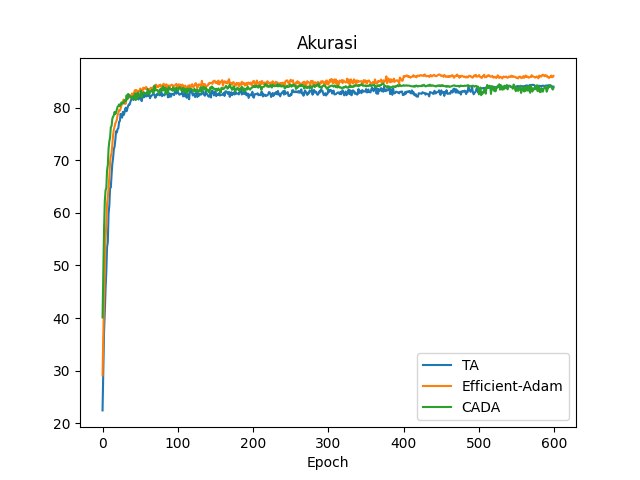
\includegraphics[width=0.8\textwidth]{acc.png}
  \caption{Akurasi tiap teknik}\label{acc}
\end{figure}

Plot perbandingan jumlah komunikasi untuk tiap teknik dapat dilihat pada gambar~\ref{comms}. Dalam plot tersebut, terlihat bahwa teknik Efficient-Adam sangat berimpitan dengan CADA. Namun, teknik CADA mampu mengurangi jumlah komunikasi dalam skala kecil, masih tetap di atas 975 komunikasi. Di sisi lain, implementasi gabungan memberikan pengurangan jumlah komunikasi yang cukup banyak, hingga hanya membutuhkan kurang dari 825 komunikasi di sebelum epoch 600.

\begin{figure}[ht]
  \centering
  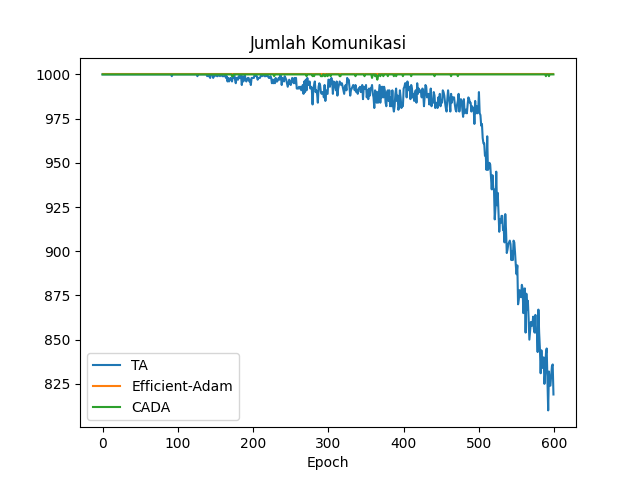
\includegraphics[width=0.8\textwidth]{comms.png}
  \caption{Jumlah komunikasi tiap teknik}\label{comms}
\end{figure}

Plot perbandingan jumlah byte yang digunakan dapat dilihat pada gambar~\ref{bits}. Dapat dilihat bahwa jumlah byte yang digunakan oleh CADA sekitar 4 kali lebih besar dibandingkan Efficient-Adam serta teknik gabungan. Namun, terlihat bahwa teknik gabungan menggunakan lebih banyak byte dibandingkan Efficient-Adam saja. Kemudian, jumlah byte yang digunakan oleh teknik gabungan terlihat berkurang sesuai dengan pengurangan jumlah komunikasi yang terjadi.

\begin{figure}[ht]
  \centering
  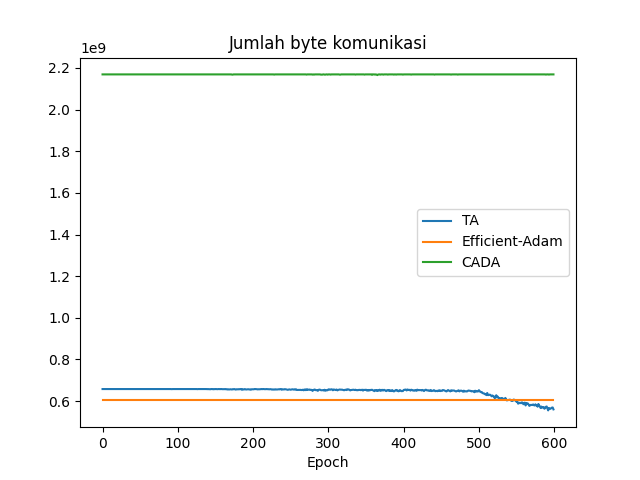
\includegraphics[width=0.8\textwidth]{bits.png}
  \caption{Jumlah byte tiap teknik}\label{bits}
\end{figure}


\subsection{Analisis Hasil Pengujian}
Berdasarkan pengujian yang dilakukan, didapatkan bahwa teknik gabungan dapat menggunakan jumlah byte lebih sedikit dibandingkan CADA, namun lebih banyak dibandingkan Efficient-Adam. Namun, teknik gabungan tetap membutuhkan sedikit lebih banyak byte untuk melakukan komunikasi dibandingkan Efficient-Adam. Penyebab meningkatnya jumlah byte adalah adanya nilai tambahan yang perlu dikomunikasikan oleh \emph{parameter server}, yakni nilai ambang yang digunakan dalam persamaan~\ref{cada2cond}.

Kemudian, jumlah komunikasi yang dilakukan oleh CADA juga masih tidak berkurang sebanyak jumlah komunikasi dalam teknik gabungan. Hal ini mungkin disebabkan karena \emph{hyperparameter} yang dipilih menyebabkan nilai selisih gradien yang didapatkan selalu besar. Dampaknya, persamaan~\ref{cada2cond} tidak pernah terpenuhi. Namun, pemilihan \emph{hyperparameter} lain, seperti menggunakan $\alpha = 0.0005$ menyebabkan model yang dihasilkan memiliki akurasi lebih rendah.

Hasil gabungan yang didapatkan memiliki akurasi yang memiliki akurasi mirip dengan kedua teknik lain. Selain itu, teknik gabungan juga mampu mengurangi kebutuhan komunikasi sejumlah 13.838 ronde dibandingkan Efficient-Adam. Kemudian, hasil gabungan juga dapat mengurangi jumlah byte yang digunakan dalam komunikasi hingga menjadi sekitar 0.303 kali dari CADA.

% \chapter{Penutup}

\section{Kesimpulan}
\begin{enumerate}
  \item Berhasil dibuat suatu teknik yang menggabungkan CADA dengan Efficient-Adam. Pengurangan komunikasi dalam teknik tersebut menggunakan ide dari CADA, sedangkan kompresi gradien menggunakan ide dari Efficient-Adam.
  \item Teknik gabungan mampu mengurangi komunikasi lebih banyak dibandingkan teknik CADA dalam skenario pelatihan model yang lebih kompleks.
  \item Teknik gabungan menggunakan lebih banyak byte untuk berkomunikasi dibandingkan teknik Efficient-Adam. Namun jumlah byte yang digunakan teknik gabungan tetap berkurang karena terdapat pengurangan jumlah komunikasi.
\end{enumerate}

\section{Saran}
\begin{enumerate}
  \item Memilih teknik lain untuk digabungkan, untuk melihat pengaruh berbagai teknik.
  \item Pengujian menggunakan model dalam ranah selain \emph{computer vision}.
  \item Pengujian menggunakan \emph{dataset} lain.
\end{enumerate}

%----------------------------------------------------------------%

% Daftar pustaka
\printbibliography
% \blankpage

% Setting judul lampiran
\titlespacing*{\chapter}{0pt}{0pt}{0pt}
\titlespacing*{\section}{0pt}{0pt}{*1}

% Setting judul anak lampiran
\titleformat*{\section}{\bfseries}

% Index
% \appendix
% \chapter{Contoh Judul Lampiran}
\section{Contoh Judul Anak Lampiran}
Here is my appendix content...
% \chapter{Contoh Judul Lampiran}
Here is my appendix content...

\end{document}
